\section{System Overview}
\label{sec:overview}

\subsection{Problem Formulation}
\label{sec:problem}

\textbf{Estimation problem.}
We estimate the continuous-time 6-DoF body trajectory (world-frame
position $\vp_w(t)\in\mathbb{R}^3$ and orientation $\vR(t)\in\SO$)
together with the constant \ac{imu} biases $\vb_a,\vb_g$, from asynchronous
measurements over \rev{a sliding estimation window}: radar Doppler velocities ($\sim$11\,Hz),
accelerometer and gyroscope samples (1\,kHz), and a low-rate heading
prior.  We adopt a \emph{continuous-time} representation because the
sensors are asynchronous and run at disparate rates: a trajectory defined
for every $t$ is evaluated at each measurement's exact timestamp, and its
derivatives (velocity $\dot{\vp}_w$, acceleration $\ddot{\vp}_w$, and
body angular velocity $\vom_b$) follow in closed form, so no
inter-sample interpolation or rigid-keyframe approximation is required.

\textbf{Parameterization.}
The position and orientation spline control points
(\autoref{sec:state}) and the \ac{imu} biases form the estimated state
\begin{equation}
  \mathcal{X} = \bigl\{\,\mathbf{P}_i,\ \vR_i,\ \vb_a,\ \vb_g\,\bigr\}.
  \label{eq:state}
\end{equation}
The radar extrinsics are fixed at their measured values.

\begin{figure}[t]
\centering
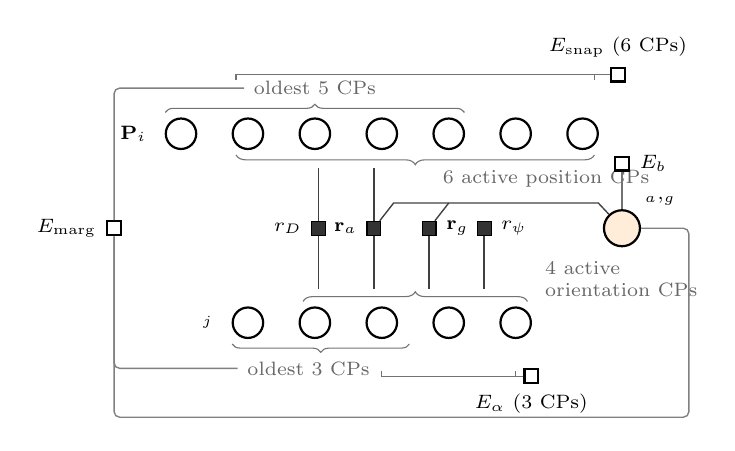
\begin{tikzpicture}[
  font=\footnotesize,
  var/.style={circle, draw, thick, fill=white, minimum size=11pt, inner sep=0pt},
  biasn/.style={circle, draw, thick, fill=orange!15, minimum size=13pt, inner sep=0pt},
  fac/.style={rectangle, draw, fill=black!80, minimum size=5pt, inner sep=0pt},
  reg/.style={rectangle, draw, thick, fill=white, minimum size=5pt, inner sep=0pt},
  edge/.style={black!75, line width=0.5pt},
  pedge/.style={black!50, line width=0.5pt, rounded corners=2pt},
  supp/.style={black!55, line width=0.5pt},
  lbl/.style={font=\scriptsize},
]
% rows: 7 position CPs, 5 orientation CPs
\foreach \i in {0,...,6}{ \node[var] (P\i) at (\i*0.85, 2.6) {}; }
\node[lbl, anchor=east] at (-0.32, 2.6) {$\mathbf{P}_i$};
\foreach \i in {0,...,4}{ \node[var] (R\i) at (0.85+\i*0.85, 0.2) {}; }
\node[lbl, anchor=east] at (0.53, 0.2) {$\vR_j$};
% active supports of the measurement factors (inner side of each row)
\draw[decorate, decoration={brace, mirror, amplitude=3.5pt}, black!55] (0.70, 2.33) -- (5.25, 2.33);
\draw[decorate, decoration={brace, amplitude=3.5pt}, black!55] (1.55, 0.47) -- (4.40, 0.47);
\node[lbl, black!60, anchor=west] at (3.2, 2.03) {6 active position CPs};
\node[lbl, black!60, anchor=west, align=left] at (4.50, 0.75) {4 active\\orientation CPs};
% measurement factors (inside both active spans)
\node[fac, label={[lbl]left:$r_{D}$}]            (fD)   at (1.75, 1.4) {};
\node[fac, label={[lbl]left:$\mathbf{r}_{a}$}]   (fa)   at (2.45, 1.4) {};
\node[fac, label={[lbl]right:$\mathbf{r}_{g}$}]  (fg)   at (3.15, 1.4) {};
\node[fac, label={[lbl]right:$r_{\psi}$}]        (fpsi) at (3.85, 1.4) {};
\draw[edge] (fD)   -- (1.75, 2.17);  \draw[edge] (fD)   -- (1.75, 0.63);
\draw[edge] (fa)   -- (2.45, 2.17);  \draw[edge] (fa)   -- (2.45, 0.63);
\draw[edge] (fg)   -- (3.15, 0.63);
\draw[edge] (fpsi) -- (3.85, 0.63);
% shared bias, right of the factor row: both IMU factors leave upward onto a
% common rail that clears the heading factor and its label
\node[biasn, label={[lbl]above right=-2pt and 0pt:$\vb_a,\vb_g$}] (b) at (5.6, 1.4) {};
\draw[edge] (fa) -- (2.70, 1.72) -- (5.30, 1.72) -- (b);
\draw[edge] (fg) -- (3.40, 1.72);
% outer side of the top row: prior (oldest 5 CPs) and min-snap (6 consecutive CPs)
\draw[decorate, decoration={brace, amplitude=3pt}, black!55] (-0.2, 2.87) -- (3.6, 2.87);
\node[lbl, black!60, anchor=south] (oldcp) at (1.7, 2.97) {oldest 5 CPs};
\draw[supp] (0.70, 3.28) -- (0.70, 3.35) -- (5.25, 3.35) -- (5.25, 3.28);
\node[reg, label={[lbl]above:$E_{\mathrm{snap}}$ (6 CPs)}] (rs) at (5.55, 3.35) {};
\draw[supp] (rs) -- (5.25, 3.35);
% outer side of the bottom row: prior (oldest 3 CPs) and angular acceleration (3 consecutive CPs)
\draw[decorate, decoration={brace, mirror, amplitude=3pt}, black!55] (0.65, -0.07) -- (2.9, -0.07);
\node[lbl, black!60, anchor=north] (oldknot) at (1.62, -0.17) {oldest 3 CPs};
\draw[supp] (2.55, -0.41) -- (2.55, -0.48) -- (4.25, -0.48) -- (4.25, -0.41);
\node[reg, label={[lbl]below:$E_{\alpha}$ (3 CPs)}] (ra) at (4.45, -0.48) {};
\draw[supp] (ra) -- (4.25, -0.48);
% bias prior: unary factor on the bias node (measured width, sec:state)
\node[reg, label={[lbl]right:$E_{b}$}] (rb) at (5.6, 2.22) {};
\draw[supp] (b) -- (rb);
% marginalization prior: oldest N-1 nodes of each row + the bias
\node[reg, label={[lbl]left:$E_{\mathrm{marg}}$}] (pr) at (-0.85, 1.4) {};
\draw[pedge] (pr) |- (oldcp.west);
\draw[pedge] (pr) |- (oldknot.west);
\draw[pedge] (pr) -- (-0.85, -1.0) -- (6.45, -1.0) -- (6.45, 1.4) -- (b);
\end{tikzpicture}
\caption{Factor graph of one measurement time $t$.
Circles are variables (position control points (CPs) $\mathbf{P}_i$,
orientation control points $\vR_j$, the shared \ac{imu} bias); filled squares
are measurement factors, open squares the regularizers and the
priors.  Each factor at time $t$ touches exactly the 6
active position CPs and/or the 4 active orientation CPs (braces): the
radar Doppler factor $r_D$ couples both splines (one such factor per
return; the returns of a frame are stacked into one block,
\autoref{sec:robust}), the accelerometer $\mathbf{r}_a$ both splines
plus the bias, the gyroscope $\mathbf{r}_g$ the orientation spline plus
the bias, the heading factor $r_\psi$ the orientation spline only.  The
minimum-snap regularizer $E_{\mathrm{snap}}$ spans 6 consecutive position CPs
and the angular-acceleration regularizer $E_\alpha$ 3 consecutive
orientation CPs; the bias prior $E_b$ anchors the bias to its pre-flight value
(\autoref{sec:state}); the marginalization prior $E_{\mathrm{marg}}$
binds the window's oldest $N{-}1$ control points of each spline and the bias
(\autoref{sec:sw}).  Not drawn: the priors of the first window (\autoref{sec:init}).  Each row
runs forward in time, but the two grids differ (40 and 16\,ms), so
horizontal positions are not aligned across rows.}
\label{fig:factorgraph}
\end{figure}

\textbf{Estimator.}
Treating the measurement noise as zero-mean and independent, the
\ac{map} estimate is the minimizer of the negative
log-posterior, a weighted nonlinear least-squares problem over the
measurement residuals, the spline regularizers, and the priors\rev{,
whose factor-graph structure \autoref{fig:factorgraph} illustrates}:
\begin{equation}
\begin{aligned}
  \hat{\mathcal{X}} = \operatorname*{arg\,min}_{\mathcal{X}}
    & \lambda_r\!\sum_{k} w_k\, r_{D,k}^2
    + \lambda_a\!\sum_{m}\lVert r_{a,m}\rVert^2 \\
    & + \lambda_g\!\sum_{m}\lVert r_{g,m}\rVert^2
    + \lambda_\psi\!\sum_{n} r_{\psi,n}^2 \\
    & + E_{\text{reg}}(\mathcal{X})
    + E_{\text{prior}}(\mathcal{X}),
\end{aligned}
\label{eq:map}
\end{equation}
where $r_D,r_a,r_g,r_\psi$ are the radar-Doppler, accelerometer,
gyroscope, and heading residuals of \autoref{sec:models}.  There is one
radar residual per return $k$, with $w_k$ the return's own weight from
the measured noise law.  The returns of a frame are stacked and
whitened for their shared error component (\autoref{sec:robust}).  The $\lambda_\bullet$ are the stream weights of \autoref{sec:char_budget}.
$E_{\text{reg}}$ collects the position min-snap and orientation
smoothness regularizers (\autoref{sec:reg}), and $E_{\text{prior}}$
collects the bias prior, the window-start priors and, online, the
marginalization prior $E_{\mathrm{marg}}$ (\autoref{sec:sw}).  We
minimize~\eqref{eq:map} with Levenberg--Marquardt using analytic
Jacobians.  The fixed-lag estimator solves it over a 3\,s window and,
on each stride, marginalizes the states leaving the window into
$E_{\mathrm{marg}}$ via the Schur complement (\autoref{sec:sw}),
keeping each window's problem size bounded.

\subsection{Hardware Platform}
The system runs on a quadrotor with a TI IWR6843AOPEVM
mmWave radar (60--64\,GHz \ac{fmcw}), the flight controller's
\ac{imu}, and a Vicon \ac{mocap} system used for ground
truth evaluation.  The radar is mounted upside-down; the extrinsic
rotation is $[180\degree, 27.5\degree, 0\degree]$
(roll, pitch, yaw) and translation $[0.08, 0.02, -0.01]$\,m in the body
frame, with the $27.5\degree$ pitch the as-built downtilt measured by
inclinometer (27--28\degree\ on the radar face).  The radar operates at $\sim$11\,Hz with 0.049\,m/s Doppler
resolution and the \ac{imu} at $\sim$993\,Hz.  Both are used at full rate.

\subsection{Pipeline}
\autoref{fig:pipeline} shows the pipeline.  A three-stage sensor-only
initialization (P1--P3, detailed in \autoref{sec:init}) builds the
initial trajectory the nonlinear solve needs, from radar and \ac{imu}
data alone.  The same raw measurements then also enter the solver directly
as factors (\autoref{fig:pipeline}, dashed).  \ac{mocap} supplies only the
yaw heading prior (a noise-free, idealized magnetometer surrogate,
whose gap to a real sensor \autoref{sec:yaw} bounds) and the final
\ac{rmse} evaluation.  P1--P3 and the position/attitude estimate use no
external pose reference.

\begin{figure}[t]
\centering
\definecolor{loopblue}{RGB}{31,119,180}
\resizebox{\columnwidth}{!}{%
\begin{tikzpicture}[
  font=\normalsize,
  box/.style={rectangle, rounded corners=3pt, draw, minimum width=1.55cm,
              minimum height=0.72cm, align=center, inner sep=2pt},
  sensor/.style={box, fill=blue!12},
  stage/.style={box, fill=orange!22},
  solver/.style={box, fill=green!16, minimum width=1.7cm, minimum height=1.05cm},
  outb/.style={box, fill=gray!12, minimum width=1.25cm},
  arr/.style={-{Latex[length=2.2mm]}, thick},
  darr/.style={-{Latex[length=2.2mm]}, thick, dashed, black!55},
  loop/.style={-{Latex[length=2.0mm]}, thick, loopblue},
  lbl/.style={font=\small},
  ]
  \node[sensor] (imu)   at (0.0,  1.6)  {\ac{imu}\\1\,kHz};
  \node[sensor] (radar) at (0.0,  0.35) {Radar\\$\sim$11\,Hz};
  \node[stage]  (p1)    at (2.35,  1.6) {P1: Gyro\\${\to}\,R(t)$};
  \node[stage]  (p2)    at (2.35,  0.35) {P2: \ac{wls}\\${\to}\,\mathbf{p}(t)$};
  \node[stage]  (p3)    at (4.35,  1.0) {P3: Priors\\${\to}$ init};
  \node[solver] (solver) at (6.35, 1.0) {Ceres\\LM solve\\{\small(sliding win.)}};
  \node[outb]   (out)   at (8.2,  1.0) {$\hat{\mathbf{p}},\,\hat{R},\,\hat{\mathbf{v}}$};
  \begin{scope}[on background layer]
    \node[draw=black!40, dashed, rounded corners=5pt, fill=orange!6,
          inner sep=6pt, fit=(p1)(p2)(p3)] (initbox) {};
    \node[lbl, black!65, anchor=south] at (initbox.north)
          {Initialization (once)};
  \end{scope}
  \draw[arr] (imu.east)   -- (p1.west);
  \draw[arr] (imu.east)   -- (p2.west);
  \draw[arr] (radar.east) -- (p2.west);
  \draw[arr] (p1.east)    -- (p3.north west);
  \draw[arr] (p2.east)    -- (p3.south west);
  \draw[arr] (p3.east)    -- (solver.west);
  \draw[arr] (solver.east)-- (out.west);
  \coordinate (busY) at (0,-0.95);
  % radar = inner bus, IMU = outer bus (no crossing)
  \draw[darr] (radar.west) -- ++(-0.32,0) |- (busY) -| (solver.south);
  \draw[darr] (imu.west) -- ++(-0.55,0) |- ($(busY)+(0,-0.42)$)
        -| ($(solver.south)+(0.25,0)$);
  \draw[loop] ([xshift=-3mm]solver.north) to[out=115,in=65,looseness=3.2]
        node[lbl, loopblue, above=0pt] {per stride}
        ([xshift=3mm]solver.north);
\end{tikzpicture}%
}% end resizebox
\caption{System pipeline. Solid: initialization flow (P1--P3 seed
the optimizer, run once). Dashed: raw sensor data fed as measurement
factors. Blue: the sliding-window re-solve at each stride.
Radar returns pass a \ac{ransac} ego-velocity prefilter
(\autoref{sec:robust}) first. \ac{mocap} supplies only the yaw heading prior
(magnetometer surrogate) and \ac{rmse} evaluation.}
\label{fig:pipeline}
\end{figure}
